\documentclass[11pt, a4paper]{article}
\usepackage[vmargin=2cm,hmargin=2cm]{geometry}
\usepackage{lipsum} 
\usepackage[utf8x]{inputenc}
\usepackage[T1]{fontenc}
\usepackage{graphicx}
\usepackage{amsmath, amsfonts}
\usepackage{amssymb, amsthm}
\usepackage[french]{babel}
\usepackage{tikz}
\usepackage{siunitx}
\usepackage{fancyhdr}
\pagestyle{fancy}
\fancyhead[L]{
\includegraphics[scale=0.2]{insa.pdf} } %pour avoir le logo de l'insa à gauche (L), le fichier insa.pdf doit se trouver dans le même dossier que le fichier tex. 
\fancyhead[C]{TPTD 2} % peut permettre d'indiquer un titre court au centre (C)
\fancyhead[R]{Auteurs : SUN Jixiang, SAMAIN Luc} % peut permettre d'indiquer le nom de l'auteur (R)
\renewcommand\headrulewidth{2pt}
\fancyfoot[C]{Page \thepage} % pour insérer le numéro de la page
\fancyfoot[R]{le 18/04/2023} % pour insérer la date  à droite (R)
\usepackage{fancybox}% pour encadrer quelques mots à l'aide de la commande \fbox

\title{Étude des interférences à l'aide d'un biprisme de Fresnel}
\author{SUN Jixiang, SAMAIN Luc}
\date{18/04/2023}

\begin{document}
\maketitle
\thispagestyle{fancy}

Le biprisme de Fresnel est un dispositif qui permet de créer à partir d'une source lumineuse, deux sources virtuelles et synchrones qui peuvent interférer entre elles. Dans ce TP-TD, on a réalisé trois expériences à l'aide d'un biprisme de Fresnel. La première utilise une source monochromatique ponctuelle placé à une distance finie. La seconde utilise la même source mais placé à l'infini. On verra que l'influence de la distance biprisme-écran est différente dans ces deux cas. Enfin, on a réalisé une expérience sur une source de lumière blanche, soit polychromatique, qui a créé les franges d'interférence colorées.

\section{Matériel}
\begin{itemize}
    \item Source Laser Nd : YAG type DPSS ($\lambda$ = 532 nm) équipé d'un objectif de microscope
    \item Biprisme de Fresnel d'indice n = 1,537 et d'angle $\alpha$ ($\approx$ 1°)
    \item Lentille convergente L (f = 100 mm)
    \item Écran d'observation
    \item Détecteur matriciel (1280$\times$1024 pixels, taille du pixel = 5,3 µm)
    \item 2 polariseurs rectilignes P1, P2
\end{itemize}


\section{Biprisme éclairé par une source ponctuelle à distance finie (ondes sphériques)}
\subsection{Protocole}
On réalise le montage de la Figure \ref{montage1}. Les polariseurs ici ne sert qu'à diminuer l'intensité de lumière pour que la caméra puisse avoir une image nette. Alors la direction des polariseurs n'a pas d'importance. La source laser crée une onde électromagnétique sphérique et, après le biprisme, elle se comporte comme deux sources virtuelles synchrones, qui vont créer un champ d'interférence triangulaire dont le sommet se situe au centre du biprisme (voir Figure \ref{champs1}). Les franges d'interférence apparaissent alors sur l'écran ou sur la caméra.

\begin{figure}[htbp]
    \centering
    \begin{minipage}[t]{0.48\textwidth}
        \centering
        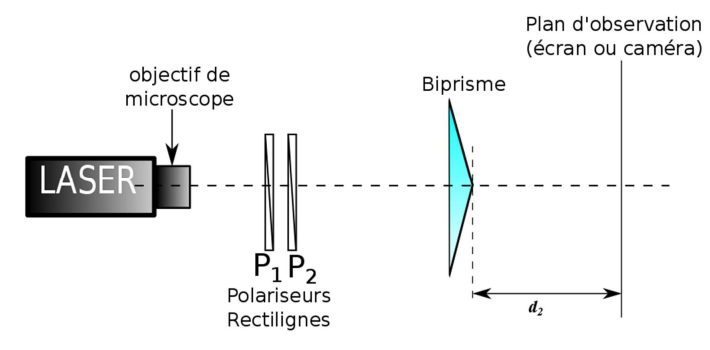
\includegraphics[width=\textwidth]{images/montage1.png}
        \caption{Schéma du dispositif expérimental permettant de visualiser les interférences entre 2 ondes sphériques}
        \label{montage1}
    \end{minipage}
    \hfill
    \begin{minipage}[t]{0.48\textwidth}
        \centering
        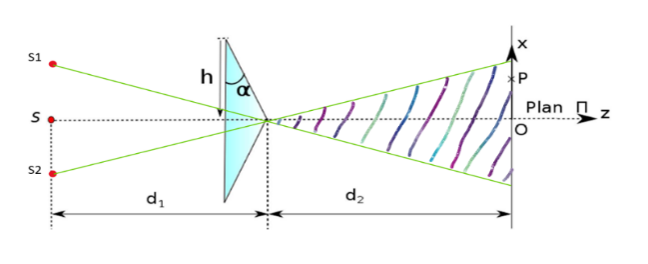
\includegraphics[width=\textwidth]{images/champs1.png}
        \caption{S1, S2 sont deux sources virtuelles et synchrones, créant un champ d'interférence triangulaire (la partie ombragée)}
        \label{champs1}
    \end{minipage}
\end{figure}
  

A l'aide de la caméra relié à un ordinateur, on peut mesurer manuellement les distances interfrange en fonction de la distance $d_2$.

La partie théorique nous dit que la distance interfrange $i$ est :

$$
    i = \frac{\lambda_0( {d_1 + d_2} )}{nS_1S_2} = \frac{\lambda_0( {d_1 + d_2} )}{2nd_1\beta} = \frac{\lambda_0( {d_1 + d_2} )}{2nd_1\left(\frac{n}{n_0}-1\right)\alpha}
$$

Où $d_1$ la distance source-biprisme, $d_2$ la distance biprisme-écran, $\beta$ la déviation du rayon, $\lambda_0$ longueur d'onde de la source dans le vide, $\alpha\approx1^{\circ}$ l'angle du biprisme, $n_v$=1,537 et $n_0$=1,0003 les indices respectifs du verre du biprisme et de l'air.

La distance interfrange $i$ a alors une relation linéaire avec $d_2$.
\subsection{Observations et résultats}
Après le montage, on observe des franges verticales, parallèles à la ligne médiane du biprisme sur l'écran. Elles sont si denses qu'il est impossible de les mesurer directement par une règle.

L'image est autant plus grande si on augmente la distance $d_2$, ainsi l'interfrange $i$. on trace alors $i=f(d_2)$ en mesurant $i$ sur l'ordinateur.

\begin{figure}[htbp]
    \centering
    \begin{minipage}[t]{0.48\textwidth}
        \centering
        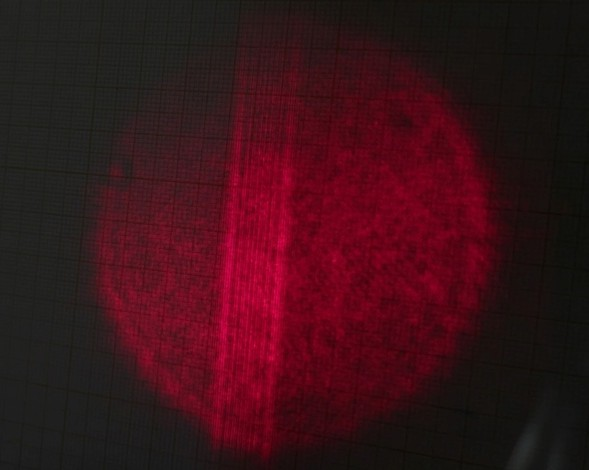
\includegraphics[width=\textwidth]{images/photo}
        \caption{les franges sur l'écran}
        \label{photo}
    \end{minipage}
    \hfill
    \begin{minipage}[t]{0.48\textwidth}
        \centering
        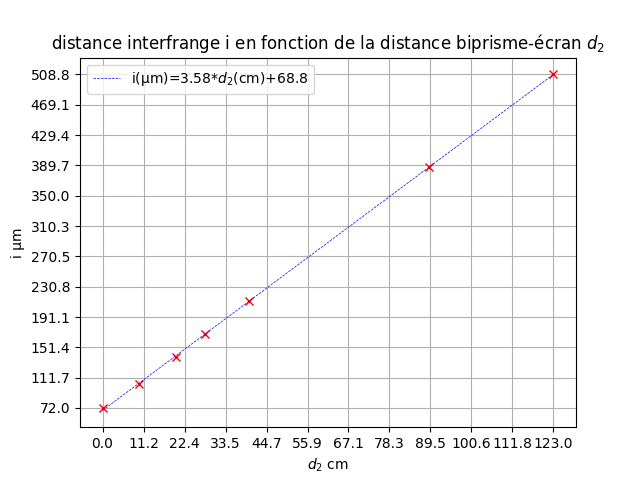
\includegraphics[width=\textwidth]{images/2.1}
        \caption{distance interfrange en fonction de la distance biprisme-écran}
        \label{courbe1}
    \end{minipage}
\end{figure}

La courbe est bien une droite qui est conforme au fait que la relation entre $i$ et $d_2$ est linéaire.


\section{Biprisme éclairé par une source ponctuelle monochromatique placée à l'infini (ondes planes)}
\subsection{Protocole}
Dans cette partie on utilise le même montage que pour l'expérience précédente à la différence où cette fois-ci on met une lentille devant le biprisme (voir Figure \ref{montage2}) et la source est au foyer de la lentille de sorte que la source se situe comme à l'infini ($d_1=\infty$) car tous les rayons reçus par le biprisme sont parallèles entre eux (onde plane).

\begin{figure}[htbp]
    \centering
    \begin{minipage}[t]{0.48\textwidth}
        \centering
        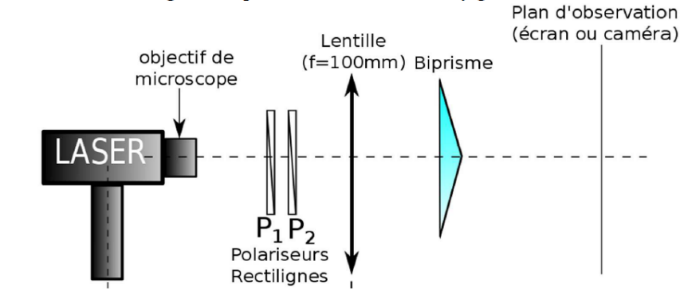
\includegraphics[width=\textwidth]{images/montage2.png}
        \caption{Schéma du dispositif expérimental permettant de visualiser les interférences entre 2 ondes planes}
        \label{montage2}
    \end{minipage}
    \hfill
    \begin{minipage}[t]{0.48\textwidth}
        \centering
        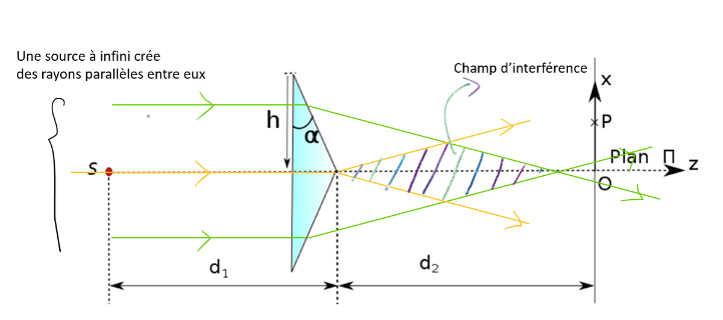
\includegraphics[width=\textwidth]{images/champs2.png}
        \caption{champ d'interférence d'une source à l'infini après le biprisme de Fresnel}
        \label{champs2}
    \end{minipage}
\end{figure}

Cette fois, le champ d'interférence est un losange (voir Figure \ref{champs2}), il existe donc une distance maximale où on peut observer les franges.

On reprend l'expression de $i$ et tend $d_1$ vers l'infini, on obtient :

$$
    i =  \frac{\lambda_0}{2n\left(\frac{n}{n_0}-1\right)\alpha}
$$

La distance interfrange est alors constante qui est indépendante de $d_1$ et de $d_2$.
\subsection{Observations et résultats}
Des franges existent toujours comme dans l'expérience précédente, mais l'image est plus petite. On trace $i$ en fonction de $d_2$ et on obtient :

\begin{figure}[h] %option h permet de mettre l'image à l'endroit indiqué
    \centering % permet de centrer l'image 
    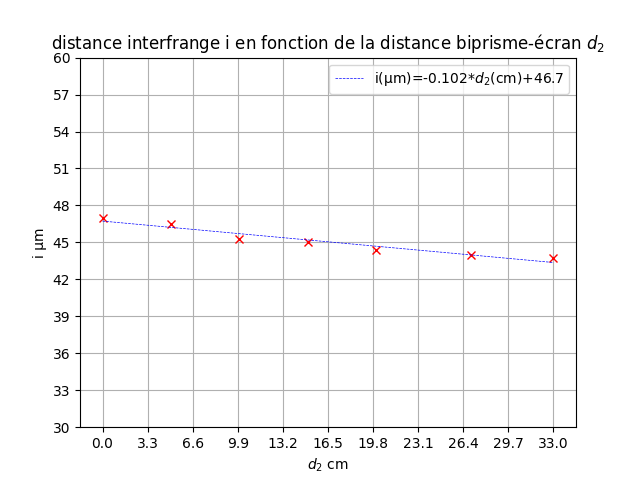
\includegraphics[width=0.75\textwidth]{images/2.2} % indiquer le nom du fichier de figure qui doit être enregistré dans le même dossier que le fichier tex, [scale=1] permet de régler la taille de la figure
    \caption{distance interfrange en fonction de la distance biprisme-écran pour la source à l'infini} % permet de donner un titre à la figure
    \label{courbe2}%donne le nom de référence de la figure qui peut être rappelée dans le texte à l'aide de \ref{insa}. Attention, il faut compiler deux fois pour que la numérotation des figures soit mise à jour dans le fichier pdf !
\end{figure}

On observe que $i$ est presque constante mais légèrement décroissante en fonction de $d_2$. On peut en déduire que la source n'est pas parfaitement au foyer de la lentille mais un peu plus loin.

Dans nos expériences, on a constaté que le nombre de franges augmente puis diminue à mesure que $d_2$ augmente et, au moment $d_2$=42 cm, il n'y a plus de franges. Cela correspondant au fait que le champ d'interférence est un losange.


\section{Interférences en lumière blanche (étude facultative)}
On réalise le montage de la Figure 8 et observe le champ. Comme auparavant, les franges d'interférences sont verticales, mais présentent cette fois un spectre de plusieurs couleurs. Cela est dû au fait que la lumière blanche est composée des lumières de différentes couleurs dans un spectre continu, qui, n'ayant pas la même longueur d'onde les unes des autres, n'interfèrent pas entre elles.

Si on regarde l'expression de la distance interfrange, on peut voir que $i$ est autant plus grande si la longueur d'onde est grande. Cela dit que pour la première frange colorée (celle la plus proche du centre), le rouge se trouve à l'extérieur et le violet à l'intérieur.

Afin de constater un maximum de couleurs différentes, il est cependant important de noter que les franges doivent être assez fines pour éviter que les différentes couleurs ne se superposent. Enfin, sur l'axe optique, la lumière est blanche car pour tout le spectre visible cette portion est constructive (la différence de marche est nulle). Nous obtenons ainsi ce qu'on appelle ‘les teintes de Newton'.

\section{Exploitation de données}
A partir de nos mesures, on peut calculer quelques valeurs. Si on injecte la moyenne de $i$ mesurée ($45,13\ \mu m$) dans la partie onde plane dans son expression pour la source à l'infini, on peut retrouver l'angle $\alpha$ de la base.

$$
    \alpha =  \frac{\lambda_0}{2n\left(\frac{n}{n_0}-1\right)i} = 0.63^\circ
$$

Ceci est conforme à la donnée que $\alpha$ est à peu près 1 degré. La déviation est alors $\beta=\left(\frac{n}{n_0}-1\right)\alpha=0.34^\circ$.

De plus, si on utilise cette valeur de $\beta$ et la pente de la figure \ref{courbe1} dans la formule de la première partie, on peut retrouver notre valeur de $d_1$ qu'on a pas pu mésurer.

$$
    d_1 =  \frac{\lambda_0}{2n\beta p} = 12.6 cm
$$
avec $p=3.58 \frac{\mu m}{cm}$ la pente de la figure \ref{courbe1}.

\section{Incertitudes et imprécisions expérimentales}
Dans ce TP, l'objectif est principalement d'observer le phénomène d'interférence et il n'y a pas de grandeur physique à déterminer. Le calcul d'incertitude n'est alors pas nécessaire. Cependant, on peut quand même évaluer les sources d'incertitude et imprécisions expérimentales afin de poser les améliorations.

Les sources d'incertitude de mesure de $d_2$ sont :
\begin{itemize}
    \item Graduation de la règle à 1mm près
    \item Lecture de valeur par opérateur
\end{itemize}

Il est à noter que l'alignement des dispositifs optiques à la flèche sur le cavalier n'est pas une source d'incertitude car on choisit arbitrairement une position comme l'origine de $d_2$, est c'est la pente de la courbe $i=f(d_2)$ qui nous intéresse.

Les sources d'incertitude de mesure de la distance d'interfrange sont :
\begin{itemize}
    \item La précision de la caméra
    \item La netteté de l'image des franges
\end{itemize}

Pour diminuer l'incertitude de $i$, on a mesuré la distance entre plusieurs franges et divisé par son nombre. Pour que l'image soit le plus nette (non surexposée ou sous-exposée), il faut bien régler les polariseurs pour avoir une intensité de lumière modérée. Le premier polariseur rend le rayon polarisé rectilignement, et on peut ensuite changer l'angle du deuxième polariseur pour régler luminosité.

\textcolor{red}{Faire + a dit la prof}

\section{Conclusion}
Ce TP-TD nous a permis d'approfondir notre compréhension des interférences lumineuses et de mettre en pratique les concepts théoriques étudiés en cours et en travaux dirigés. Les différentes expériences réalisées ont illustré la manière dont les interférences dépendent de la nature des ondes incidentes (sphériques ou planes) et de la source lumineuse utilisée (monochromatique ou polychromatique). Enfin, la comparaison de nos résultats expérimentaux avec la théorie a renforcé notre confiance dans la validité des principes fondamentaux des interférences lumineuses.
\end{document}